% Cover letter using letter.cls
\documentclass[a4paper]{scrreprt} 
%\usepackage{helvetica} % uses helvetica postscript font (download helvetica.sty)
%\usepackage{newcent}   % uses new century schoolbook postscript font 
\usepackage[utf8]{inputenc}
\usepackage{graphicx}
\usepackage{eurosym}
% the following commands control the margins:
%\topmargin=-1in    % Make letterhead start about 1 inch from top of page 
%\textheight=8.5in    % text height can be bigger for a longer letter
%\oddsidemargin=0pt   % leftmargin is 1 inch
%\textwidth=6.5in     % textwidth of 6.5in leaves 1 inch for right margin
\title{Implementing a temperature and humidity sensor network for the nEDM
experiment setup}
\author{Wenwen Chen, Rainer Schönberger}
\begin{document}
\maketitle
\tableofcontents
\input{Concept}
\section{Features}
\section{Sensors}
\subsection{TSIC 506F}
For temperature measurements, we use the TSIC 506F temperature sensor
integrated circuit. At a relatively low proce of about \EUR{7} per device, it
is able to deliver very high accuracy (see table \ref{tab:tsic}).\\
The temperature is converted to a digital value, which is sent out over a
proprietary one wire protocol variant, called \emph{ZAC} (details see section \ref{chap:zac}).

\begin{table}[H!]
	\centering
	\begin{tabular}{| r | c |}
		\hline
		Temperature range & $-10\,^{\circ}\mathrm{C}$ to $-10\,^{\circ}\mathrm{C}$\\
		\hline
		Calibrated accuracy & $\pm 0.1\,\mathrm{K}$  \\
		\hline
		Resolution & $0.034\,\mathrm{K}$  \\
		\hline
	\end{tabular}
	\caption{TSIC 506F specs}
	\label{tab:tsic}
\end{table}
\subsection{HYT271}
\section{Logical design}
\begin{figure}
	\centering
	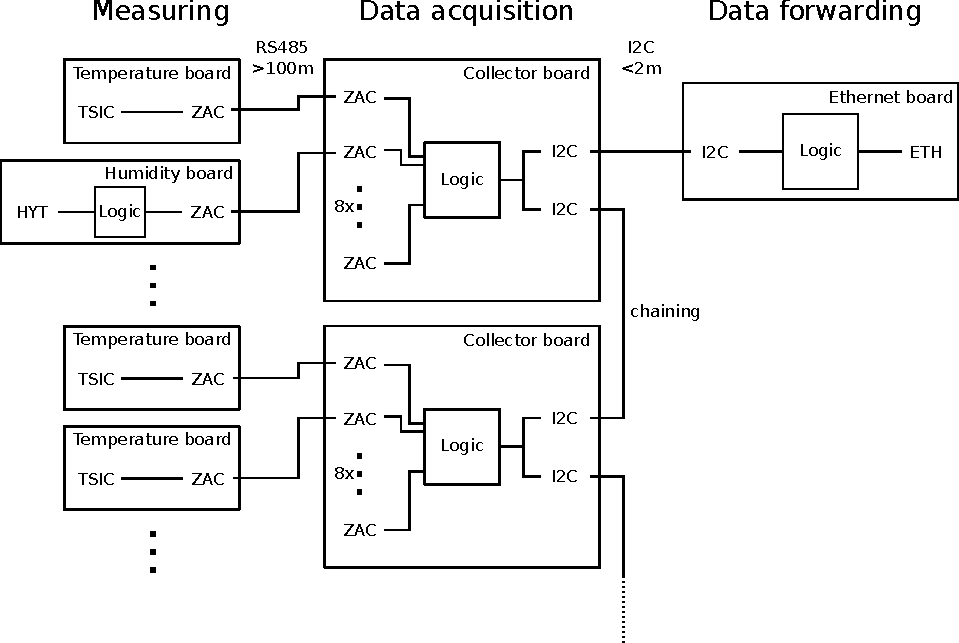
\includegraphics[width=0.9\textwidth]{img/plan2.pdf}
	\caption{Network topology}
	\label{fig:topo}
\end{figure}
\section{Protocols}
\subsection{ZAC}\label{chap:zac}
\begin{figure}
	\centering
	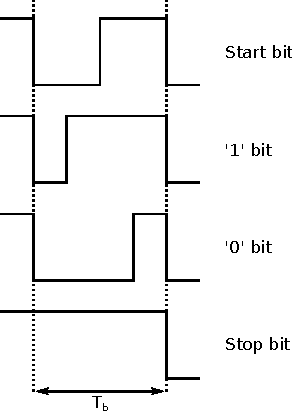
\includegraphics[width=0.3\textwidth]{img/zac_bits.pdf}
	\caption{ZAC protocol signal interpretation}
	\label{fig:zac}
\end{figure}
\begin{figure}
	\centering
	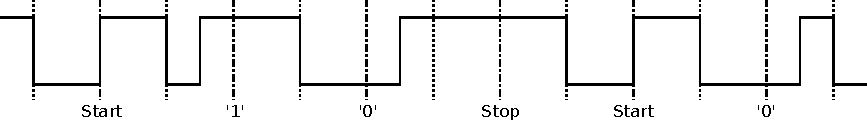
\includegraphics[width=0.9\textwidth]{img/zac_example.pdf}
	\caption{ZAC protocol example}
	\label{fig:zacexample}
\end{figure}
\subsection{I2C}
\subsection{RS485}
\input{Implementation}
\section{Temperature board}
\begin{figure}
	\centering
	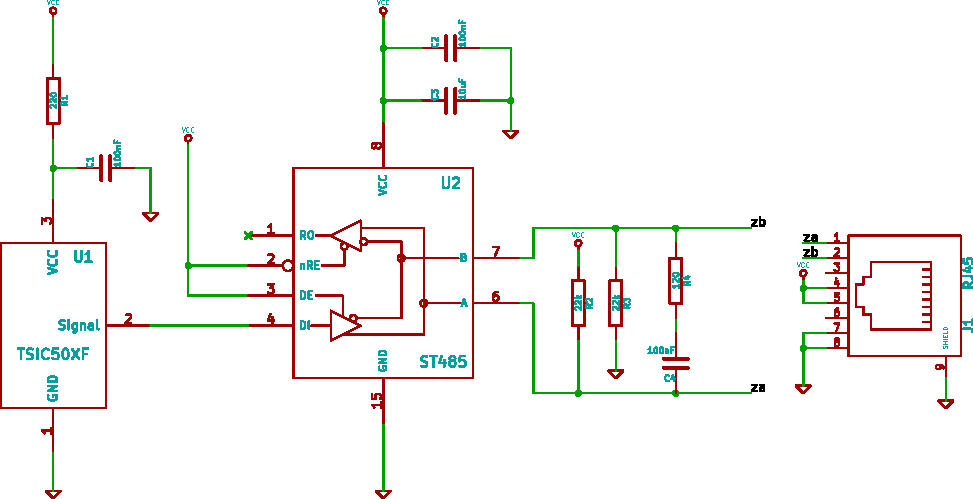
\includegraphics[width=0.6\textwidth]{img/schem_temperature_board.pdf}
	\caption{Temperature board schematic}
	\label{fig:schem_temp}
\end{figure}
\section{Humidity board}
\subsection{Hardware}
\begin{figure}
	\centering
	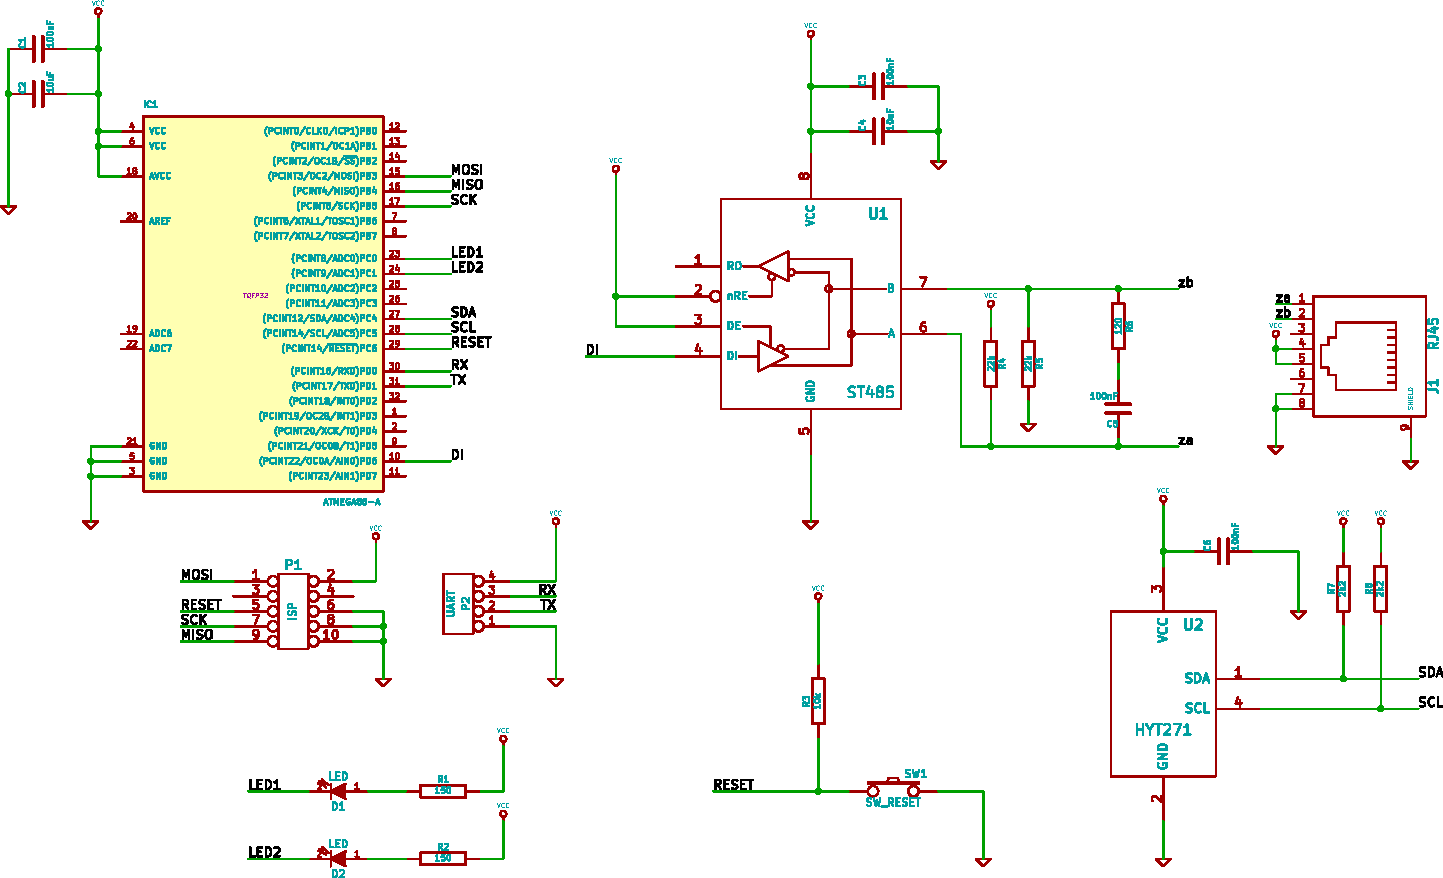
\includegraphics[width=0.8\textwidth]{img/schem_humidity_board.pdf}
	\caption{Humidity board schematic}
	\label{fig:schem_hum}
\end{figure}
\subsection{Software}
\section{Collector board}
\subsection{Hardware}
\begin{figure}
	\centering
	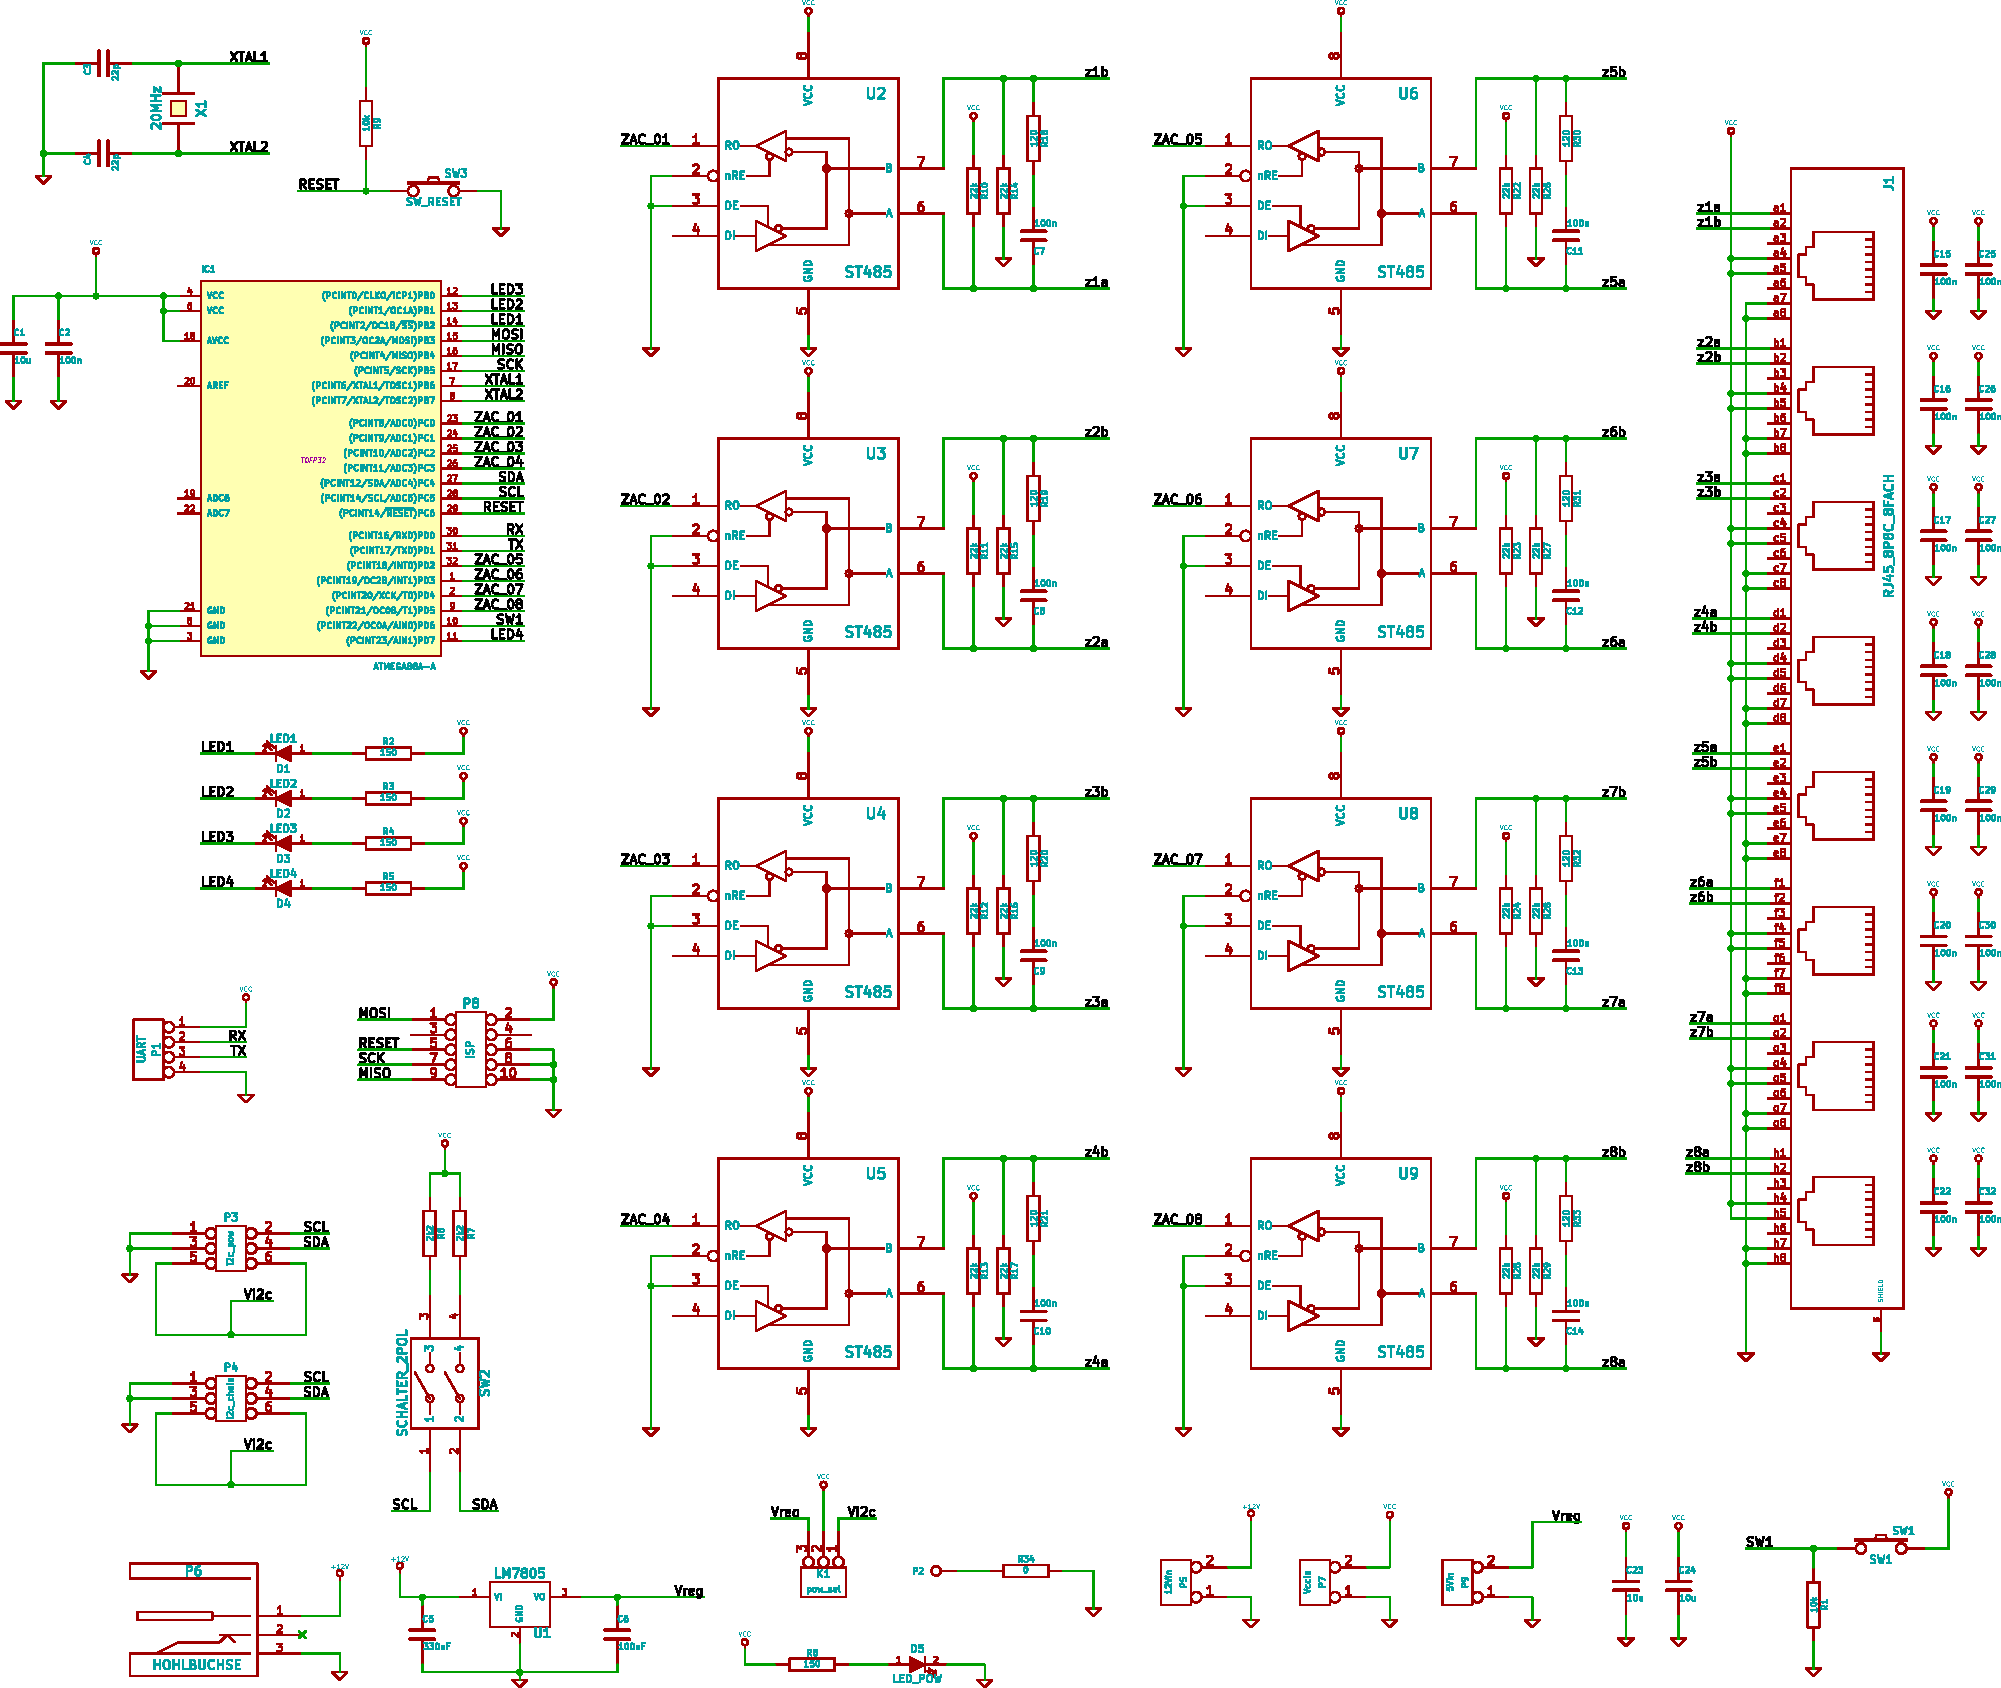
\includegraphics[width=1\textwidth]{img/schem_collector_board.pdf}
	\caption{Collector board schematic}
	\label{fig:schem_collect}
\end{figure}
\subsection{Software}
\begin{figure}
	\centering
	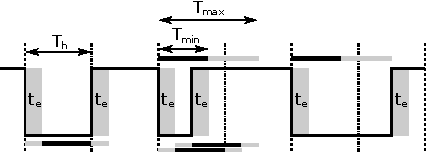
\includegraphics[width=0.7\textwidth]{img/zac_timing.pdf}
	\caption{ZAC protocol worst case timing}
	\label{fig:zactiming}
\end{figure}
\section{Ethernet board}
\subsection{Hardware}
\subsection{Software}
\subsection{User interface}
\chapter{Deployment}

\input{Conclusion}
\end{document}
